% journal_results_coverage.tex — results subsection on the validity of the
% surrogate contribution. Numbers: results/journal/summary.json
% ("coverage", "coverage_ranges"); see paper/NUMBERS_journal.md.

\subsection{Is the surrogate contribution valid?}
\label{sec:res-coverage}
Fig.~\ref{fig:coverage} and Table~\ref{tab:coverage} test the three models of
the surrogate error of Section~\ref{sec:contrib} against the true models, for
every surrogate fitted to 20 runs (68 combinations of model and surrogate on
the eleven analytical models, 30 seeds each).

\emph{Pointwise intervals.} The jackknife+ interval covered between 95.2\%
and 99.6\% of the test points (median 97.4\%) in every combination, in line
with its distribution-free guarantee of at least 90\%. The CV-normal interval
covered 89.7--97.1\% (median 94.2\%). The GP's own predictive interval
covered 68--98\% (median 88\%) and fell below 80\% on the plume (both
input models), Ishigami, piston, wing weight and 20-input OTL models: its
posterior SD reflects the fitted covariance, not the actual error. Validity
has a price in width: jackknife+ intervals were a median 1.6 (1.1--2.9)
times as wide as CV-normal ones, and the narrow GP intervals still had the
best interval score~\cite{gneiting2007} in 31 of the 49 GP combinations. For a measurement
uncertainty statement, which claims a coverage probability, the coverage is
the property that matters.

\emph{GUM S1 coverage interval.} Treating the surrogate as exact gave
coverage intervals for $Y$ whose achieved coverage under the reference
distribution ranged from 57\% to 96\% (median 94\%), and standard
uncertainties $u(y)$ that were a median 0.95 times the reference (down to
0.41). Adding the LOO error to every Monte Carlo trial,
equation~\eqref{eq:contrib}, raised the achieved coverage to 91.5--97.3\%
(median 94.9\%) as a normal error and to 91.0--97.0\% (median 94.9\%) by
resampling the residuals, with $u(y)$ a median 1.00 (0.78--1.29) times the
reference. The GP's predictive SD gave 89.8--96.0\% (median 94.6\%). The
largest correction occurred where it is needed most: for the GP with the
original kernel on the Ishigami model, coverage rose from 57\% to 95\%.
Adding the error did not systematically improve exceedance probabilities,
which depend on the tail of the surrogate rather than on its overall
spread.

\emph{Reported quantities.} The difference between the approaches is
largest for the quantities a GUM~S1 evaluation reports. Intervals for
$y_{0.95}$ from joint GP posterior sample paths contained the true value in
a median 63\% of seeds (7--100\%), and those for $P(Y>T)$ in 63\%: the GP
posterior describes the uncertainty of the interpolant as the fitted
covariance model sees it, and is overconfident wherever that model is
misspecified. The jackknife intervals contained the true value in a median
97\% of seeds for both quantities, with the lowest values for the
original-kernel GP, whose error is a bias that no resampling of its own
fits can reveal.

\begin{figure*}[tb]
\centering
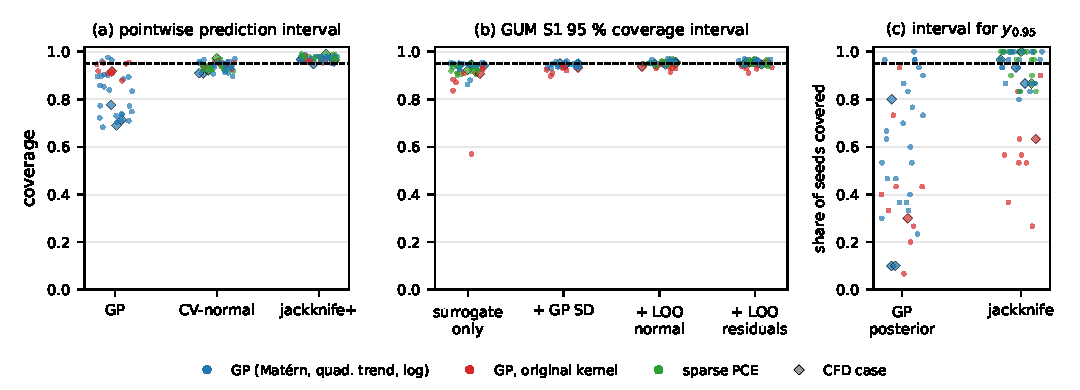
\includegraphics[width=\textwidth]{journal/fig_coverage}
\caption{Coverage of nominal 95\% intervals, mean over 30 seeds; one marker
per combination of model and surrogate (circles: the eleven analytical
models; diamonds: the CFD case, Section~\ref{sec:res-cfd}).
(a) Pointwise prediction intervals on 5000 test points. (b) Achieved
coverage of the GUM~S1 95\% coverage interval of $Y$ under the reference
distribution, with the surrogate treated as exact or with its error added
to each trial. (c) Share of seeds whose 95\% interval for $y_{0.95}$
contains the true value. Dashed line: 0.95.}
\label{fig:coverage}
\end{figure*}

\begin{table*}[tb]
\centering
\caption{Coverage (\%) of nominal 95\% intervals for the GP recommended for
each model (log variables for positive outputs), 30 seeds, $N=20$.
Pointwise: share of test points. GUM~S1: achieved coverage of the 95\%
coverage interval of $Y$. $y_{0.95}$, $P(Y>T)$: share of seeds whose
interval contains the true value (GP: joint posterior paths; J: jackknife).
Generated from the result records.}
\label{tab:coverage}
\scriptsize
\setlength{\tabcolsep}{3.5pt}
\begin{tabular}{l rrr rrrr rr rr}
\toprule
& \multicolumn{3}{c}{Pointwise} & \multicolumn{4}{c}{GUM S1 interval of $Y$} &
\multicolumn{2}{c}{$y_{0.95}$} & \multicolumn{2}{c}{$P(Y>T)$}\\
\cmidrule(lr){2-4}\cmidrule(lr){5-8}\cmidrule(lr){9-10}\cmidrule(lr){11-12}
Model & GP & CV & J+ & exact & +LOO N & +LOO res. & +GP & GP & J & GP & J\\
\midrule
\tabinput{../results/journal/tab_coverage.tex}
\bottomrule
\end{tabular}
\end{table*}

\subsection{Robustness of the surrogate contribution}
\label{sec:res-robust}
\emph{Hyperparameter uncertainty.} Integrating out the GP's hyperparameters
narrowed the gap but did not close it (Table~\ref{tab:bayesgp}). Over the 42
combinations of model and GP candidate at $N=20$, the median pointwise
coverage rose from 80\% with the plug-in hyperparameters to 83\% for the
Student-t process and 96\% for the fully Bayesian GP; the recalibrated GP
reached 95\% (91--98\%) and the jackknife+ 97\%. For the reported quantities
the gain was smaller. Intervals for $y_{0.95}$ contained the true value in
at least 26 of the 30 seeds, the threshold fixed in advance, in 13 of the 42
combinations with the plug-in GP, 15 with the Student-t process, 24 with
the fully Bayesian GP, 23 with the recalibrated GP and 39 with the
jackknife. The fully Bayesian GP fell as low as 8 of 30 seeds (Mat\'ern GP
on the CFD case): averaging over hyperparameters cannot repair a covariance
model that does not fit the response, here the raw scale of a positive,
skewed output. The jackknife fell short of the threshold on three
combinations, all raw-scale GPs on the plume model with GUM-type inputs
and on the Ishigami model (24--25 of 30). By the rule fixed in advance,
none of the GP-based descriptions is a valid surrogate contribution on all
models, and the recommendation of the LOO residuals stands. The coverage
interval of $Y$ itself was robust to the choice: 93\% or more with every
error model. The MCMC chains had integrated autocorrelation times of 38--62
steps, so the 500 steps kept per walker span 8--13 autocorrelation times.

\emph{Number of runs.} The procedure (the candidate with the smallest LOO
error in each seed, with its LOO residuals added) gave GUM~S1 coverage
intervals that covered 93.4--96.9\% of the reference distribution at
$N=10$, 94.2--96.1\% at 20, 94.7--95.7\% at 40 and 94.7--95.1\% at 80, on
every model (Table~\ref{tab:budgets}). Treating the chosen surrogate as
exact covered as little as 81.9\% at $N=10$, against 89.9\% at 20: the
contribution matters most when the budget is smallest. With ten runs, a
design's coverage fell below 90\% in up to 23\% of the designs of a model,
with 20 runs in at most 3\% and with 40 or 80 runs in none. The selection
was within 4.4\% of the best candidate in hindsight at every budget from 20
runs, but up to 37\% worse at $N=10$, where ten LOO residuals rank the
candidates less reliably. A 95\% jackknife+ interval needs at least 19 runs;
with ten it is unbounded. The jackknife intervals for $y_{0.95}$ contained
the true value in 19--30 of 30 seeds at $N=10$ and 23--30 at $N=40$. At
$N=80$ they did so in 14 of 30 seeds on the physics model, whose surrogate
error at that budget (a relative error of $y_{0.95}$ below $10^{-4}$) is at
the level of the observation noise shared by all LOO fits, which no
resampling of the fits can reveal.

\emph{Single designs.} A practitioner has one design. At $N=20$, with the
LOO residuals added, the achieved coverage of the GUM~S1 interval was below
90\% in at most 10\% of the designs of any model and surrogate (median 0\%),
and never below 80.8\%.

\emph{A feature the runs miss.} On the bump model, 13 of the 30 designs of
20 runs placed a run inside the bump. When the design missed it, the GUM~S1
interval still covered 94--95\% of the reference distribution, because the
bump holds only 3\% of the probability mass, and the jackknife+ intervals
95--97\% of the test points; but the intervals for $y_{0.95}$ contained the
true value in only 9--10 of the 17 designs, against 13 of 13 when the bump
was hit. With 40 runs, 6 designs missed the bump, and their intervals for
$y_{0.95}$ contained the true value in 1--4 of 6. Nothing computed from the
runs can flag this: the LOO residuals, like every estimate from the runs,
describe only the errors that the runs reveal. A local feature smaller than
the spacing of the design needs prior knowledge of where to look, or runs
placed there.

\begin{table*}[tb]
\centering
\caption{GP-based descriptions of the surrogate error against the
jackknife, $N=20$, for the GP with a quadratic trend on the recommended
scale (log for positive outputs). Pointwise: mean coverage (\%) of 95\%
prediction intervals on the test points. $y_{0.95}$: seeds (of 30) whose
95\% interval for the 95th percentile contains the true value. Plug-in: ML
hyperparameters; t: Student-t process; MCMC: all hyperparameters
integrated out; recal.: GP SD recalibrated by the LOO standardised
residuals; J+/J: jackknife+ and jackknife. Generated from the result
records.}
\label{tab:bayesgp}
\scriptsize
\setlength{\tabcolsep}{3.2pt}
\begin{tabular}{l rrrrr rrrrr}
\toprule
& \multicolumn{5}{c}{Pointwise coverage (\%)} & \multicolumn{5}{c}{$y_{0.95}$: seeds of 30 covered}\\
\cmidrule(lr){2-6}\cmidrule(lr){7-11}
Model & plug-in & t & MCMC & recal. & J+ & plug-in & t & MCMC & recal. & J\\
\midrule
\tabinput{../results/journal/tab_bayesgp.tex}
\bottomrule
\end{tabular}
\end{table*}

\begin{table}[tb]
\centering
\caption{Achieved coverage (\%) of the GUM~S1 95\% coverage interval of $Y$
for the procedure (candidate chosen by LOO error, LOO residuals added),
mean over 30 seeds, against the number of runs. The CFD case was not run
with 80 runs. Generated from the result records.}
\label{tab:budgets}
\small
\begin{tabular}{l rrrr}
\toprule
Model & $N=10$ & 20 & 40 & 80\\
\midrule
\tabinput{../results/journal/tab_budgets.tex}
\bottomrule
\end{tabular}
\end{table}
